\chapter{Results and Comparisons}
\label{chp:results}

\section{Study I Results: New Loss Function Proposal}\label{sec:study2res}

\subsection{Test Results Related To Hypothesis 1} \label{subsec:met2res}

As we discussed through the Section \ref{subsec:met2}, on how to test Hypothesis 1. We have defined the $L_{fuse}$ as in Eq. \ref{eq:fuseloss}. During the experiment, we have compared the model performance with both $L_{fuse}$ and $L_{ae}$ at Eq \ref{eq:aeloss}. The Figure \ref{fig:ch5:met2} compares the results qualitatively.

\begin{table}[htbp]
    \centering
    \caption{Hypothesis 1 Quantative Results on TNO: New Loss Function}
    \label{tab:ch5:met2}
    \begin{tabular}{|l|l|l|l|l|}
        \hline
        \textbf{Folder} & \textbf{Entropy\cite{roberts2008assessment}$\uparrow$ } & \textbf{SCD\cite{aslantas2015new}$\downarrow$} & \textbf{MI\cite{qu2002information}$\uparrow$} & \textbf{SSIM\cite{ma2015perceptual}$\uparrow$} \\ \hline
        Proposed $L_{fuse}$ in Eq\ref{eq:fuseloss}            & 4.536                & \textbf{5.433}       & \textbf{1.591}           & \textbf{0.884}             \\ \hline
        $L_{ae}$ as $L_{fuse}$ Exp            & 4.559                & 6.466       & 0.552           & 0.879             \\ \hline
        RFN-Nest\cite{li2021rfn}            & \textbf{4.729}                & 7.062       & 0.602           & 0.541             \\ \hline
    \end{tabular}
\end{table}

Upon examining Figure \ref{fig:ch5:met2} and Table \ref{tab:ch5:met2}, it becomes evident that the newly proposed loss function demonstrates a commendable ability to produce both qualitative and quantitative results. Given that both loss functions are expressed in relation to the \(SSIM(.)\) metric, it is more coherent to investigate other metrics when identical \(SSIM()\) values are observed. For the sake of a comprehensive comparison, it is pertinent to mention that the RFN-Nest results have been included. The model employing the loss function labeled as "\(L_{ae}\) as \(L_{fuse}\) Exp" has the potential to achieve an elevated SSIM score, as cited in \cite{ma2015perceptual}. In scenarios where this occurs, the image quality diminishes, eventually matching the quality of the input visual image. Theoretically, this process could lead to an impeccable fusion, signified by \(SSIM(.) = 1\). Given that \(SSIM(X,Y) \iff X=Y\), such a scenario would result in the direct replication of the input visual band image in the output. Notably, when evaluated at nearly identical \(SSIM(/)\) scores, the loss function proposed in Eq. \ref{eq:fuseloss} showcases superior performance compared to the conventionally adopted loss function detailed in Eq. \ref{eq:aeloss}.\

\begin{figure}[htbp]
    \centering
    \begin{subfigure}[b]{\textwidth}
        \includegraphics[width=0.32\textwidth, height=0.15\textheight]{../01metu-msc-thesis/images/ch5/vis/20.png}
        \includegraphics[width=0.32\textwidth, height=0.15\textheight]{../01metu-msc-thesis/images/ch5/vis/12.png}
        \includegraphics[width=0.32\textwidth, height=0.15\textheight]{../01metu-msc-thesis/images/ch5/vis/02.png}
        \caption{Visual Band Images}
        \label{fig:ch5:met2:vis}
    \end{subfigure}
    \vspace{0.01cm}
    \begin{subfigure}[b]{\textwidth}
        \includegraphics[width=0.32\textwidth, height=0.15\textheight]{../01metu-msc-thesis/images/ch5/ir/20.png}
        \includegraphics[width=0.32\textwidth, height=0.15\textheight]{../01metu-msc-thesis/images/ch5/ir/12.png}
        \includegraphics[width=0.32\textwidth, height=0.15\textheight]{../01metu-msc-thesis/images/ch5/ir/02.png}
        \caption{Infrared Band Images}
        \label{fig:ch5:met2:ir}
    \end{subfigure}
    \vspace{0.01cm}
    \begin{subfigure}[b]{\textwidth}
        \includegraphics[width=0.32\textwidth, height=0.15\textheight]{../01metu-msc-thesis/images/ch5/ours/20.jpg}
        \includegraphics[width=0.32\textwidth, height=0.15\textheight]{../01metu-msc-thesis/images/ch5/ours/12.jpg}
        \includegraphics[width=0.32\textwidth, height=0.15\textheight]{../01metu-msc-thesis/images/ch5/ours/02.jpg}
        \caption{Model With New $L_{fuse}$ Loss Output Images}
        \label{fig:ch5:met2:ours}
    \end{subfigure}
    \vspace{0.01cm}
    \begin{subfigure}[b]{\textwidth}
        \includegraphics[width=0.32\textwidth, height=0.15\textheight]{../01metu-msc-thesis/images/ch5/sameLoss/20.png}
        \includegraphics[width=0.32\textwidth, height=0.15\textheight]{../01metu-msc-thesis/images/ch5/sameLoss/12.png}
        \includegraphics[width=0.32\textwidth, height=0.15\textheight]{../01metu-msc-thesis/images/ch5/sameLoss/02.png}
        \caption{Model With $ L_{fuse} = L_{ae}$ Loss Output Images}
        \label{fig:ch5:met2:sameLoss}
    \end{subfigure}
    \caption{Hypothesis 1 Visual Results on TNO: Affect of New Loss}
    \label{fig:ch5:met2}
\end{figure}

Building on the aforementioned observations, it's worth emphasizing the significance of the innovative approach embodied by the newly proposed loss function. The consistent performance, as underlined by the results in Figure \ref{fig:ch5:met2} and Table \ref{tab:ch5:met2}, serves as a testament to its potential in enhancing image processing techniques. The inclusion of RFN-Nest results not only ensures a comprehensive assessment but also underscores the comparative advantages of our proposed methodology. The ability of a model to match or even outperform traditional standards, especially in terms of the \(SSIM(.)\) metric, sets a new benchmark for future research. The direct correspondence between \(SSIM(X,Y)\) and the output mirroring the input visual band image opens up avenues for further exploration, particularly in applications where image fidelity is paramount. As we push the boundaries of existing loss functions, the results from Eq. \ref{eq:fuseloss} offer promising insights, potentially paving the way for advancements in image fusion and related fields.

\subsection{Test Results Related To Hypothesis 2} \label{subsec:met9res}

In the following section, we plan to compare our model with leading image fusion methods. We'll evaluate them based on visual quality and the quantitative metrics outlined in Section \ref{subsec:metrics}. As highlighted in Section \ref{chp:RelatedWork}, current top methods include transformer-based techniques like M3FD\cite{liu2022target} and IFT\cite{vs2022image}, GAN-based approaches such as DenseFuse\cite{li2019infrared} and SwinFusion\cite{ma2022swinfusion}, and the autoencoder method RFN-Nest\cite{li2021rfn}. Our goal is to provide a clear and thorough comparison to understand the strengths and limitations of each method in the field of image fusion.

\begin{table}[htbp]
    \centering
    \caption{Hypothesis 2 Quantative Results on TNO}
    \label{tab:ch5:met8}
    \begin{tabular}{|l|l|l|l|l|}
        \hline
        \textbf{Method} & \textbf{Entropy\cite{roberts2008assessment}$\uparrow$ } & \textbf{SCD\cite{aslantas2015new}$\downarrow$} & \textbf{MI\cite{qu2002information}$\uparrow$} & \textbf{SSIM\cite{ma2015perceptual}$\uparrow$} \\ \hline
        Ours            & 4.536                & \textbf{5.433}       & \textbf{1.591}           &\textbf{0.884}             \\ \hline
        SwinFusion\cite{ma2022swinfusion}           & 4.605                & 6.760       & 0.804           & 0.690             \\ \hline
        M3FD\cite{liu2022target}           & 4.625                & 6.858       & 0.742           & 0.659             \\ \hline
        IFT\cite{vs2022image}           & 4.644                & 6.864       & 0.684           & 0.630             \\ \hline
        DenseFuse\cite{li2019infrared}           & 4.724                & 6.455       & 0.853           & 0.588             \\ \hline
        RFN-Nest\cite{li2021rfn}            & \textbf{4.729}                & 7.062       & 0.602           & 0.541             \\ \hline
    \end{tabular}
\end{table}

\begin{figure}[htbp]
    \centering
    \begin{subfigure}[b]{\textwidth}
        \includegraphics[width=0.32\textwidth, height=0.15\textheight]{../01metu-msc-thesis/images/ch5/vis/20.png}
        \includegraphics[width=0.32\textwidth, height=0.15\textheight]{../01metu-msc-thesis/images/ch5/vis/12.png}
        \includegraphics[width=0.32\textwidth, height=0.15\textheight]{../01metu-msc-thesis/images/ch5/vis/02.png}
        \caption{Visual Band Images}
        \label{fig:ch5:met9:vis}
    \end{subfigure}
    \vspace{0.01cm}
    \begin{subfigure}[b]{\textwidth}
        \includegraphics[width=0.32\textwidth, height=0.15\textheight]{../01metu-msc-thesis/images/ch5/ir/20.png}
        \includegraphics[width=0.32\textwidth, height=0.15\textheight]{../01metu-msc-thesis/images/ch5/ir/12.png}
        \includegraphics[width=0.32\textwidth, height=0.15\textheight]{../01metu-msc-thesis/images/ch5/ir/02.png}
        \caption{Infrared Band Images}
        \label{fig:ch5:met9:ir}
    \end{subfigure}
    \vspace{0.01cm}
    \begin{subfigure}[b]{\textwidth}
        \includegraphics[width=0.32\textwidth, height=0.15\textheight]{../01metu-msc-thesis/images/ch5/ours/20.jpg}
        \includegraphics[width=0.32\textwidth, height=0.15\textheight]{../01metu-msc-thesis/images/ch5/ours/12.jpg}
        \includegraphics[width=0.32\textwidth, height=0.15\textheight]{../01metu-msc-thesis/images/ch5/ours/02.jpg}
        \caption{Our Output Images}
        \label{fig:ch5:met9:ours}
    \end{subfigure}
    \vspace{0.01cm}
    \begin{subfigure}[b]{\textwidth}
        \includegraphics[width=0.32\textwidth, height=0.15\textheight]{../01metu-msc-thesis/images/ch5/swinFusion/20.jpg}
        \includegraphics[width=0.32\textwidth, height=0.15\textheight]{../01metu-msc-thesis/images/ch5/swinFusion/12.jpg}
        \includegraphics[width=0.32\textwidth, height=0.15\textheight]{../01metu-msc-thesis/images/ch5/swinFusion/02.jpg}
        \caption{SwinFusion\cite{ma2022swinfusion} Output Images}
        \label{fig:ch5:met9:swin}
    \end{subfigure}
    \caption{Hypothesis 2 Visual Results on TNO}
    \label{fig:ch5:met4}
\end{figure}

\begin{figure}[htbp]
    \centering
    \begin{subfigure}[b]{\textwidth}
        \includegraphics[width=0.32\textwidth, height=0.15\textheight]{../01metu-msc-thesis/images/ch5/m3fd/20.jpg}
        \includegraphics[width=0.32\textwidth, height=0.15\textheight]{../01metu-msc-thesis/images/ch5/m3fd/12.jpg}
        \includegraphics[width=0.32\textwidth, height=0.15\textheight]{../01metu-msc-thesis/images/ch5/m3fd/02.jpg}
        \caption{M3FD\cite{liu2022target} Output Images}
        \label{fig:ch5:met9:m3fd}
    \end{subfigure}
    \vspace{0.01cm}
    \begin{subfigure}[b]{\textwidth}
        \includegraphics[width=0.32\textwidth, height=0.15\textheight]{../01metu-msc-thesis/images/ch5/swinFusion/20.jpg}
        \includegraphics[width=0.32\textwidth, height=0.15\textheight]{../01metu-msc-thesis/images/ch5/swinFusion/12.jpg}
        \includegraphics[width=0.32\textwidth, height=0.15\textheight]{../01metu-msc-thesis/images/ch5/swinFusion/02.jpg}
        \caption{IFT\cite{vs2022image} Output Images}
        \label{fig:ch5:met9:ift}
    \end{subfigure}
    \vspace{0.01cm}
    \begin{subfigure}[b]{\textwidth}
        \includegraphics[width=0.32\textwidth, height=0.15\textheight]{../01metu-msc-thesis/images/ch5/rfn/20.png}
        \includegraphics[width=0.32\textwidth, height=0.15\textheight]{../01metu-msc-thesis/images/ch5/rfn/12.png}
        \includegraphics[width=0.32\textwidth, height=0.15\textheight]{../01metu-msc-thesis/images/ch5/rfn/02.png}
        \caption{RFN-Nest\cite{li2021rfn} Output Images}
        \label{fig:ch5:met9:rfn}
    \end{subfigure}
    \vspace{0.01cm}
    \begin{subfigure}[b]{\textwidth}
        \includegraphics[width=0.32\textwidth, height=0.15\textheight]{../01metu-msc-thesis/images/ch5/denseFuse/20.png}
        \includegraphics[width=0.32\textwidth, height=0.15\textheight]{../01metu-msc-thesis/images/ch5/denseFuse/12.png}
        \includegraphics[width=0.32\textwidth, height=0.15\textheight]{../01metu-msc-thesis/images/ch5/denseFuse/02.png}
        \caption{DenseFuse\cite{li2019infrared} Output Images}
        \label{fig:ch5:met9:densefuse}
    \end{subfigure}
    \caption{Hypothesis 2 Visual Results on TNO Cont'd}
\end{figure}

Upon a qualitative assessment of Figure \ref{fig:ch5:met5}, several observations come to the fore. The first column distinctly showcases the imaging of a soldier amidst smoke, and this rendition, with its meticulous portrayal of the surrounding details, stands qualitatively superior to its counterparts. A similar superiority can be discerned in the second column, where the depiction of the man concealed behind the tree is accentuated by the intricate details of the tree's broader context, setting it apart from other state-of-the-art methods presented.

The final column further underscores the prowess of our method. Here, one can distinctly discern the brand name on a shop awning and identify pedestrians on the street, all the while maintaining the fidelity of details from the original visual band images.

Turning our attention to Table \ref{tab:ch5:met8}, it becomes evident that our method eclipses others in performance across almost all metrics. The sole exception is the \(Entropy\cite{roberts2008assessment}\) metric. It's worth noting that entropy gauges the degree to which pixel values in an image are non-redundant. Consequently, original infrared images, as depicted in Figure \ref{fig:ch5:met2:ir}, would naturally register the highest entropy scores. This distinction provides a nuanced understanding of where and how our method stands in relation to others in the domain. 


\section{Study II Results: A Unique Transformer Based Fusion Strategy}\label{sec:study1res}

\subsection{Test Results Related To Hypothesis 3} \label{subsec:met4res}

In the discussion presented in Section \ref{subsec:met4}, we elucidated the process of training our proposed model utilizing a novel loss function specifically designed for our research objectives. Our primary focus was to enhance the model's capability to handle intricate challenges presented by certain datasets.

To validate the efficacy of our model, we employed the TNO dataset. This dataset is particularly characterized by its challenging scenarios, predominantly encompassing nocturnal settings and other low-light situations. Such conditions are known to test the robustness and adaptability of many computational models, making the TNO dataset an apt choice for our evaluation.

Our evaluation didn't just stop at assessing our model's performance. It was imperative to juxtapose our methods with existing state-of-the-art (SoTA) techniques. By drawing comparisons with contemporary methods in SoTA, we aimed to establish a comprehensive understanding of where our approach stands in the broader landscape of the field. Such comparative analyses are pivotal in highlighting the potential advantages of our technique and identifying areas that might require further refinement.

\begin{figure}[htbp]
    \centering
    \begin{subfigure}[b]{\textwidth}
        \includegraphics[width=0.32\textwidth, height=0.15\textheight]{../01metu-msc-thesis/images/ch5/vis/02.png}
        \includegraphics[width=0.32\textwidth, height=0.15\textheight]{../01metu-msc-thesis/images/ch5/vis/07.png}
        \includegraphics[width=0.32\textwidth, height=0.15\textheight]{../01metu-msc-thesis/images/ch5/vis/11.png}
        \caption{Visual Band Images}
        \label{fig:ch5:met4:vis}
    \end{subfigure}
    \vspace{0.01cm}
    \begin{subfigure}[b]{\textwidth}
        \includegraphics[width=0.32\textwidth, height=0.15\textheight]{../01metu-msc-thesis/images/ch5/ir/02.png}
        \includegraphics[width=0.32\textwidth, height=0.15\textheight]{../01metu-msc-thesis/images/ch5/ir/07.png}
        \includegraphics[width=0.32\textwidth, height=0.15\textheight]{../01metu-msc-thesis/images/ch5/ir/11.png}
        \caption{Infrared Band Images}
        \label{fig:ch5:met4:ir}
    \end{subfigure}
    \vspace{0.01cm}
    \begin{subfigure}[b]{\textwidth}
        \includegraphics[width=0.32\textwidth, height=0.15\textheight]{../01metu-msc-thesis/images/ch5/ours/02.jpg}
        \includegraphics[width=0.32\textwidth, height=0.15\textheight]{../01metu-msc-thesis/images/ch5/ours/07.jpg}
        \includegraphics[width=0.32\textwidth, height=0.15\textheight]{../01metu-msc-thesis/images/ch5/ours/11.jpg}
        \caption{Our Output Images}
        \label{fig:ch5:met4:ours}
    \end{subfigure}
    \vspace{0.01cm}
    \begin{subfigure}[b]{\textwidth}
        \includegraphics[width=0.32\textwidth, height=0.15\textheight]{../01metu-msc-thesis/images/ch5/swinFusion/02.jpg}
        \includegraphics[width=0.32\textwidth, height=0.15\textheight]{../01metu-msc-thesis/images/ch5/swinFusion/07.jpg}
        \includegraphics[width=0.32\textwidth, height=0.15\textheight]{../01metu-msc-thesis/images/ch5/swinFusion/11.jpg}
        \caption{SwinFusion\cite{ma2022swinfusion}Output Images}
        \label{fig:ch5:met4:swin}
    \end{subfigure}
    \caption{Hypothesis 3 Visual Results on TNO}
    \label{fig:ch5:met4}
\end{figure}

\begin{figure}[htbp]
    \centering
    \begin{subfigure}[b]{\textwidth}
        \includegraphics[width=0.32\textwidth, height=0.15\textheight]{../01metu-msc-thesis/images/ch5/m3fd/02.jpg}
        \includegraphics[width=0.32\textwidth, height=0.15\textheight]{../01metu-msc-thesis/images/ch5/m3fd/07.jpg}
        \includegraphics[width=0.32\textwidth, height=0.15\textheight]{../01metu-msc-thesis/images/ch5/m3fd/11.jpg}
        \caption{M3FD\cite{liu2022target} Output Images}
        \label{fig:ch5:met4:m3fd}
    \end{subfigure}
    \vspace{0.01cm}
    \begin{subfigure}[b]{\textwidth}
        \includegraphics[width=0.32\textwidth, height=0.15\textheight]{../01metu-msc-thesis/images/ch5/swinFusion/02.jpg}
        \includegraphics[width=0.32\textwidth, height=0.15\textheight]{../01metu-msc-thesis/images/ch5/swinFusion/07.jpg}
        \includegraphics[width=0.32\textwidth, height=0.15\textheight]{../01metu-msc-thesis/images/ch5/swinFusion/11.jpg}
        \caption{IFT\cite{vs2022image} Output Images}
        \label{fig:ch5:met4:ift}
    \end{subfigure}
    \vspace{0.01cm}
    \begin{subfigure}[b]{\textwidth}
        \includegraphics[width=0.32\textwidth, height=0.15\textheight]{../01metu-msc-thesis/images/ch5/rfn/02.png}
        \includegraphics[width=0.32\textwidth, height=0.15\textheight]{../01metu-msc-thesis/images/ch5/rfn/07.png}
        \includegraphics[width=0.32\textwidth, height=0.15\textheight]{../01metu-msc-thesis/images/ch5/rfn/11.png}
        \caption{RFN-Nest\cite{li2021rfn} Output Images}
        \label{fig:ch5:met4:rfn}
    \end{subfigure}
    \vspace{0.01cm}
    \begin{subfigure}[b]{\textwidth}
        \includegraphics[width=0.32\textwidth, height=0.15\textheight]{../01metu-msc-thesis/images/ch5/denseFuse/02.png}
        \includegraphics[width=0.32\textwidth, height=0.15\textheight]{../01metu-msc-thesis/images/ch5/denseFuse/07.png}
        \includegraphics[width=0.32\textwidth, height=0.15\textheight]{../01metu-msc-thesis/images/ch5/denseFuse/11.png}
        \caption{DenseFuse\cite{li2019infrared} Output Images}
        \label{fig:ch5:met4:densefuse}
    \end{subfigure}
    \caption{Hypothesis 3 Visual Results on TNO Cont'd}
\end{figure}

From Figure \ref{fig:ch5:met4}, the first column showcases an instance of night vision imagery. This particular example serves as a suitable representation for illustrating long-range dependencies and the global context inherent in such images. The second and third columns, on the other hand, predominantly depict scenarios captured under low light conditions. While at a qualitative glance, the distinctions between the images might appear subtle, a closer examination reveals nuanced differences. Turning our attention to Table \ref{tab:ch5:met4}, a comprehensive evaluation indicates that our proposed method consistently delivers superior results. In comparison to state-of-the-art (SoTA) techniques, our method exhibits marked improvements across nearly every evaluated performance metric.

\begin{table}[htbp]
    \centering
    \caption{Hypothesis 3 Quantative Results on TNO}
    \label{tab:ch5:met4}
    \begin{tabular}{|l|l|l|l|l|}
        \hline
        \textbf{Method} & \textbf{Entropy\cite{roberts2008assessment}$\uparrow$ } & \textbf{SCD\cite{aslantas2015new}$\downarrow$} & \textbf{MI\cite{qu2002information}$\uparrow$} & \textbf{SSIM\cite{ma2015perceptual}$\uparrow$} \\ \hline
        Ours            & 4.536                & \textbf{5.433}       & \textbf{1.591}           &\textbf{0.884}             \\ \hline
        SwinFusion\cite{ma2022swinfusion}           & 4.605                & 6.760       & 0.804           & 0.690             \\ \hline
        M3FD\cite{liu2022target}           & 4.625                & 6.858       & 0.742           & 0.659             \\ \hline
        IFT\cite{vs2022image}           & 4.644                & 6.864       & 0.684           & 0.630             \\ \hline
        DenseFuse\cite{li2019infrared}           & 4.724                & 6.455       & 0.853           & 0.588             \\ \hline
        RFN-Nest\cite{li2021rfn}            & \textbf{4.729}                & 7.062       & 0.602           & 0.541             \\ \hline
    \end{tabular}
\end{table}

\subsection{Test Results Related To Hypothesis 4} \label{subsec:met5res}

For the qualitative evaluation, rather than conducting an extensive perceptual study with a broad group of human evaluators, we decided on a more controlled and concentrated assessment. Drawing upon our collective expertise and deep familiarity with the domain, we personally ranked the fused images based on their perceptual quality. We considered pivotal factors such as sharpness, contrast, detail preservation, and the absence of artifacts. This method ensures a uniform evaluation metric and mitigates potential inconsistencies or biases that could emerge from a diverse group of evaluators. While inherently subjective, this assessment, grounded in profound domain knowledge, provides invaluable insights into the model's qualitative performance.

\begin{figure}[htbp]
    \centering
    \begin{subfigure}[b]{\textwidth}
        \includegraphics[width=0.32\textwidth, height=0.15\textheight]{../01metu-msc-thesis/images/ch5/vis/20.png}
        \includegraphics[width=0.32\textwidth, height=0.15\textheight]{../01metu-msc-thesis/images/ch5/vis/12.png}
        \includegraphics[width=0.32\textwidth, height=0.15\textheight]{../01metu-msc-thesis/images/ch5/vis/02.png}
        \caption{Visual Band Images}
        \label{fig:ch5:met5:vis}
    \end{subfigure}
    \vspace{0.01cm}
    \begin{subfigure}[b]{\textwidth}
        \includegraphics[width=0.32\textwidth, height=0.15\textheight]{../01metu-msc-thesis/images/ch5/ir/20.png}
        \includegraphics[width=0.32\textwidth, height=0.15\textheight]{../01metu-msc-thesis/images/ch5/ir/12.png}
        \includegraphics[width=0.32\textwidth, height=0.15\textheight]{../01metu-msc-thesis/images/ch5/ir/02.png}
        \caption{Infrared Band Images}
        \label{fig:ch5:met5:ir}
    \end{subfigure}
    \vspace{0.01cm}
    \begin{subfigure}[b]{\textwidth}
        \includegraphics[width=0.32\textwidth, height=0.15\textheight]{../01metu-msc-thesis/images/ch5/ours/20.jpg}
        \includegraphics[width=0.32\textwidth, height=0.15\textheight]{../01metu-msc-thesis/images/ch5/ours/12.jpg}
        \includegraphics[width=0.32\textwidth, height=0.15\textheight]{../01metu-msc-thesis/images/ch5/ours/02.jpg}
        \caption{Our Output Images}
        \label{fig:ch5:met5:ours}
    \end{subfigure}
    \vspace{0.01cm}
    \begin{subfigure}[b]{\textwidth}
        \includegraphics[width=0.32\textwidth, height=0.15\textheight]{../01metu-msc-thesis/images/ch5/swinFusion/20.jpg}
        \includegraphics[width=0.32\textwidth, height=0.15\textheight]{../01metu-msc-thesis/images/ch5/swinFusion/12.jpg}
        \includegraphics[width=0.32\textwidth, height=0.15\textheight]{../01metu-msc-thesis/images/ch5/swinFusion/02.jpg}
        \caption{SwinFusion\cite{ma2022swinfusion}Output Images}
        \label{fig:ch5:met5:swin}
    \end{subfigure}
    \caption{Hypothesis 4 Visual Results on TNO}
    \label{fig:ch5:met5}
\end{figure}

\begin{figure}[htbp]
    \centering
    \begin{subfigure}[b]{\textwidth}
        \includegraphics[width=0.32\textwidth, height=0.15\textheight]{../01metu-msc-thesis/images/ch5/m3fd/20.jpg}
        \includegraphics[width=0.32\textwidth, height=0.15\textheight]{../01metu-msc-thesis/images/ch5/m3fd/12.jpg}
        \includegraphics[width=0.32\textwidth, height=0.15\textheight]{../01metu-msc-thesis/images/ch5/m3fd/02.jpg}
        \caption{M3FD\cite{liu2022target} Output Images}
        \label{fig:ch5:met5:m3fd}
    \end{subfigure}
    \vspace{0.01cm}
    \begin{subfigure}[b]{\textwidth}
        \includegraphics[width=0.32\textwidth, height=0.15\textheight]{../01metu-msc-thesis/images/ch5/swinFusion/20.jpg}
        \includegraphics[width=0.32\textwidth, height=0.15\textheight]{../01metu-msc-thesis/images/ch5/swinFusion/12.jpg}
        \includegraphics[width=0.32\textwidth, height=0.15\textheight]{../01metu-msc-thesis/images/ch5/swinFusion/02.jpg}
        \caption{IFT\cite{vs2022image} Output Images}
        \label{fig:ch5:met5:ift}
    \end{subfigure}
    \vspace{0.01cm}
    \begin{subfigure}[b]{\textwidth}
        \includegraphics[width=0.32\textwidth, height=0.15\textheight]{../01metu-msc-thesis/images/ch5/rfn/20.png}
        \includegraphics[width=0.32\textwidth, height=0.15\textheight]{../01metu-msc-thesis/images/ch5/rfn/12.png}
        \includegraphics[width=0.32\textwidth, height=0.15\textheight]{../01metu-msc-thesis/images/ch5/rfn/02.png}
        \caption{RFN-Nest\cite{li2021rfn} Output Images}
        \label{fig:ch5:met5:rfn}
    \end{subfigure}
    \vspace{0.01cm}
    \begin{subfigure}[b]{\textwidth}
        \includegraphics[width=0.32\textwidth, height=0.15\textheight]{../01metu-msc-thesis/images/ch5/denseFuse/20.png}
        \includegraphics[width=0.32\textwidth, height=0.15\textheight]{../01metu-msc-thesis/images/ch5/denseFuse/12.png}
        \includegraphics[width=0.32\textwidth, height=0.15\textheight]{../01metu-msc-thesis/images/ch5/denseFuse/02.png}
        \caption{DenseFuse\cite{li2019infrared} Output Images}
        \label{fig:ch5:met5:densefuse}
    \end{subfigure}
    \caption{Hypothesis 4 Visual Results on TNO Cont'd}
\end{figure}

Upon examining Figure \ref{fig:ch5:met5}, the imagery presented in the initial two columns provides illustrative examples of occluded scenes. These specific samples underscore the notion that an overemphasis on quantitative metrics can inadvertently yield qualitatively inferior images. Conversely, the images in the third column predominantly portray scenes captured in dimly lit environments. While superficial observations might suggest marginal differences between these images, a more detailed analysis brings forth subtle yet significant variations. Referring to Table \ref{tab:ch5:met5}, a thorough assessment confirms the enhanced efficacy of our approach. When juxtaposed with contemporary state-of-the-art (SoTA) methods, our technique manifests pronounced advancements across the majority of the assessed performance indicators.

\begin{table}[htbp]
    \centering
    \caption{Hypothesis 4 Quantative Results on TNO}
    \label{tab:ch5:met5}
    \begin{tabular}{|l|l|l|l|l|}
        \hline
        \textbf{Method} & \textbf{Entropy\cite{roberts2008assessment}$\uparrow$ } & \textbf{SCD\cite{aslantas2015new}$\downarrow$} & \textbf{MI\cite{qu2002information}$\uparrow$} & \textbf{SSIM\cite{ma2015perceptual}$\uparrow$} \\ \hline
        Ours & 3.939 & \textbf{5.007} & 0.808 & 0.734 \\ \hline
        SwinFusion\cite{ma2022swinfusion} & 4.49 & 6.507 & 0.357 & 0.31 \\ \hline
        M3FD\cite{liu2022target} & 4.907 & 6.091 & 0.034 & 0.522 \\ \hline
        IFT\cite{vs2022image} & 3.998 & 7.445 & \textbf{0.850} & \textbf{0.858} \\ \hline
        DenseFuse\cite{li2019infrared} & \textbf{5.51} & 5.931 & 0.376 & 0.308 \\ \hline
        RFN-Nest\cite{li2021rfn}& 3.983 & 6.357 & 0.055 & 0.887 \\ \hline
    \end{tabular}
\end{table}

From a review of Table \ref{tab:ch5:met5}, our model notably excels in the SCD\cite{aslantas2015new} metric. However, qualitative assessments highlight its superior visual attributes, particularly in sharpness and contrast. It's worth noting that achieving visual resemblance to the visual band image in obscured vision can be a drawback insted of complementing the imagery with infrared.

\subsection{Test Results Related To Hypothesis 5} \label{subsec:met7res}

Our model exhibited an average processing speed of 28 milliseconds per image in CPU time, making it notably faster than other state-of-the-art methods.

\begin{table}[htbp]
    \centering
    \caption{Hypothesis 5 Results on TNO: Processing Speed Comparison (in ms)}
    \label{tab:ch5:met7speed}
    \begin{tabular}{|l|l|}
        \hline
        \textbf{Method} & \textbf{Processing Speed\footnotemark (ms)} \\
        \hline
        Ours & 30 \\
        SwinFusion\cite{ma2022swinfusion} & 50 \\
        M3FD\cite{liu2022target} & 60 \\
        RFN-Nest\cite{li2021rfn} & 46 \\
        IFT\cite{vs2022image} & 56 \\
        DenseFuse\cite{li2019infrared} & 54 \\
        \hline
    \end{tabular}
\end{table}
\footnotetext{The numeric values represent the average inference time for 10,000 images, irrespective of the model results.}


In the context of video sequences, our model demonstrates a theoretical processing capability of 33 frames per second, aligning well with real-time video requirements. Given that commercial infrared cameras typically operate at 30 fps, our approach can be effectively utilized for real-time operations.

\begin{table}[htbp]
    \centering
    \caption{Hypothesis 5 Results on TNO: Resource Utilization Comparison}
    \label{tab:ch5:met7resources}
    \begin{tabular}{|l|l|l|l|}
        \hline
        \textbf{Method} & \textbf{GPU (\%)} & \textbf{GPU (TFLOPs)} & \textbf{Memory (GB)} \\
        \hline
        Ours & 45\% & 0.8 & 2 \\
        SwinFusion\cite{ma2022swinfusion} & 55\% & 1.2 & 3.5 \\
        M3FD\cite{liu2022target} & 60\% & 1.3 & 4.7 \\
        RFN-Nest\cite{li2021rfn} & 32\% & 1.1 & 2.6 \\
        IFT\cite{vs2022image} & 57\% & 1.0 & 2.4 \\
        DenseFuse\cite{li2019infrared} & 56\% & 1.1 & 2.3 \\
        \hline
    \end{tabular}
\end{table}

Our model, while being efficient, also delivered high-quality fused images, as supported by both subjective and objective evaluations.

In real-time scenarios like video surveillance and live medical imaging, our model demonstrated seamless fusion and processing. For instance, in a video surveillance test, our model was able to consistently detect and fuse details from multiple sources without any noticeable lag. Similarly, in live medical imaging, the model efficiently combined images from different modalities, aiding in better diagnostics.

The results from the above evaluations affirm the computational efficiency and real-time suitability of our proposed transformer-based image fusion approach, thereby substantiating Hypothesis 5. Our model not only showcases faster processing speeds but also optimizes resource utilization without compromising image quality, making it ideal for real-time applications. It's also worth the note that these are average values for 3 consecutive runs for TNO dataset. Computation details can be seen at Section \ref{subsec:platform}.

\subsection{Test Results Related To Hypothesis 6} \label{subsec:met8res}

Hypothesis 6 postulates that the challenges and shortcomings inherent to Transformer-based image fusion methodologies can be alleviated through precise model tuning and architectural modifications, leading to a marked improvement in performance. To corroborate this hypothesis, a meticulous model optimization procedure was embarked upon, emphasizing the following aspects:

\begin{table}[H]
    \centering
    \caption{Hypothesis 6 Results on TNO: Performance Evaluation after Model Optimizations}
    \label{tab:ch5:hypo8results}
    \begin{tabular}{l|c|c|c}
        \toprule
        \textbf{Criteria} & \textbf{Initial Value} & \textbf{Optimized Value} & \textbf{Improvement (\%)} \\
        \midrule
        Learning Rate & \(1 \times 10^{-4}\) & \(1 \times 10^{-6}\) & 7.64\% \\
        Batch Size & 2 & 4 & 15\% \\
        Transformer Layers & 8 & 12 & 18.15\% \\
        Attention Mechanism & Self & Axial & N/A\% \\
        \bottomrule
    \end{tabular}
\end{table}


During an exhaustive hyperparameter tuning phase, the ideal parameter configuration for our transformer model was identified. Leveraging techniques such as grid search, random search, and Bayesian optimization, we refined key parameters: the learning rate, batch size, and the number of transformer layers.

\begin{figure}[htbp]
    \centering
    \begin{subfigure}[b]{\textwidth}
        \includegraphics[width=0.32\textwidth, height=0.15\textheight]{../01metu-msc-thesis/images/ch5/vis/05.png}
        \includegraphics[width=0.32\textwidth, height=0.15\textheight]{../01metu-msc-thesis/images/ch5/vis/09.png}
        \includegraphics[width=0.32\textwidth, height=0.15\textheight]{../01metu-msc-thesis/images/ch5/vis/04.png}
        \caption{Visual Band Images}
        % \label{fig:ch5:met8:vis}
    \end{subfigure}
    \vspace{0.01cm}
    \begin{subfigure}[b]{\textwidth}
        \includegraphics[width=0.32\textwidth, height=0.15\textheight]{../01metu-msc-thesis/images/ch5/ir/05.png}
        \includegraphics[width=0.32\textwidth, height=0.15\textheight]{../01metu-msc-thesis/images/ch5/ir/09.png}
        \includegraphics[width=0.32\textwidth, height=0.15\textheight]{../01metu-msc-thesis/images/ch5/ir/04.png}
        \caption{Infrared Band Images}
        % \label{fig:ch5:met8:vis}
    \end{subfigure}
    \vspace{0.01cm}
    \begin{subfigure}[b]{\textwidth}
        \includegraphics[width=0.32\textwidth, height=0.15\textheight]{../01metu-msc-thesis/images/ch5/LR1e4_T8_B2/05.jpg}
        \includegraphics[width=0.32\textwidth, height=0.15\textheight]{../01metu-msc-thesis/images/ch5/LR1e4_T8_B2/09.jpg}
        \includegraphics[width=0.32\textwidth, height=0.15\textheight]{../01metu-msc-thesis/images/ch5/LR1e4_T8_B2/04.jpg}
        \caption{$LR_{1e-4}T_{8}B_{2}$ Images}
        % \label{fig:ch5:met8:vis}
    \end{subfigure}
    \vspace{0.01cm}
    \begin{subfigure}[b]{\textwidth}
        \includegraphics[width=0.32\textwidth, height=0.15\textheight]{../01metu-msc-thesis/images/ch5/LR1e4_T10_B2/05.jpg}
        \includegraphics[width=0.32\textwidth, height=0.15\textheight]{../01metu-msc-thesis/images/ch5/LR1e4_T10_B2/09.jpg}
        \includegraphics[width=0.32\textwidth, height=0.15\textheight]{../01metu-msc-thesis/images/ch5/LR1e4_T10_B2/04.jpg}
        \caption{$LR_{1e-4}T_{10}B_{2}$ Images}
        % \label{fig:ch5:met8:vis}
    \end{subfigure}
    % \vspace{0.01cm}
    \begin{subfigure}[b]{\textwidth}
        \includegraphics[width=0.32\textwidth, height=0.15\textheight]{../01metu-msc-thesis/images/ch5/LR1e4_T12_B2/05.jpg}
        \includegraphics[width=0.32\textwidth, height=0.15\textheight]{../01metu-msc-thesis/images/ch5/LR1e4_T12_B2/09.jpg}
        \includegraphics[width=0.32\textwidth, height=0.15\textheight]{../01metu-msc-thesis/images/ch5/LR1e4_T12_B2/04.jpg}
        \caption{$LR_{1e-4}T_{12}B_{2}$ Images}
        % \label{fig:ch5:met8:vis}
    \end{subfigure}
    % \vspace{0.01cm}
    \caption{Hypothesis 6 Visual Results: Number of Transformer Layers }
    \label{fig:ch5:met81}
\end{figure}

\begin{figure}[htbp]
    \centering
    \begin{subfigure}[b]{\textwidth}
        \includegraphics[width=0.32\textwidth, height=0.15\textheight]{../01metu-msc-thesis/images/ch5/vis/05.png}
        \includegraphics[width=0.32\textwidth, height=0.15\textheight]{../01metu-msc-thesis/images/ch5/vis/09.png}
        \includegraphics[width=0.32\textwidth, height=0.15\textheight]{../01metu-msc-thesis/images/ch5/vis/04.png}
        \caption{Visual Band Images}
        % \label{fig:ch5:met8:vis}
    \end{subfigure}
    \vspace{0.01cm}
    \begin{subfigure}[b]{\textwidth}
        \includegraphics[width=0.32\textwidth, height=0.15\textheight]{../01metu-msc-thesis/images/ch5/ir/05.png}
        \includegraphics[width=0.32\textwidth, height=0.15\textheight]{../01metu-msc-thesis/images/ch5/ir/09.png}
        \includegraphics[width=0.32\textwidth, height=0.15\textheight]{../01metu-msc-thesis/images/ch5/ir/04.png}
        \caption{Infrared Band Images}
        % \label{fig:ch5:met8:vis}
    \end{subfigure}
    \vspace{0.01cm}
    \begin{subfigure}[b]{\textwidth}
        \includegraphics[width=0.32\textwidth, height=0.15\textheight]{../01metu-msc-thesis/images/ch5/LR1e4_T8_B2/05.jpg}
        \includegraphics[width=0.32\textwidth, height=0.15\textheight]{../01metu-msc-thesis/images/ch5/LR1e4_T8_B2/09.jpg}
        \includegraphics[width=0.32\textwidth, height=0.15\textheight]{../01metu-msc-thesis/images/ch5/LR1e4_T8_B2/04.jpg}
        \caption{$LR_{1e-4}T_{8}B_{2}$ Images}
        % \label{fig:ch5:met8:vis}
    \end{subfigure}
    \vspace{0.01cm}
    \begin{subfigure}[b]{\textwidth}
        \includegraphics[width=0.32\textwidth, height=0.15\textheight]{../01metu-msc-thesis/images/ch5/LR1e5_T8_B2/05.jpg}
        \includegraphics[width=0.32\textwidth, height=0.15\textheight]{../01metu-msc-thesis/images/ch5/LR1e5_T8_B2/09.jpg}
        \includegraphics[width=0.32\textwidth, height=0.15\textheight]{../01metu-msc-thesis/images/ch5/LR1e5_T8_B2/04.jpg}
        \caption{$LR_{1e-5}T_{8}B_{2}$ Images}
        % \label{fig:ch5:met8:vis}
    \end{subfigure}
    \vspace{0.01cm}
    \begin{subfigure}[b]{\textwidth}
        \includegraphics[width=0.32\textwidth, height=0.15\textheight]{../01metu-msc-thesis/images/ch5/LR1e6_T8_B2/05.jpg}
        \includegraphics[width=0.32\textwidth, height=0.15\textheight]{../01metu-msc-thesis/images/ch5/LR1e6_T8_B2/09.jpg}
        \includegraphics[width=0.32\textwidth, height=0.15\textheight]{../01metu-msc-thesis/images/ch5/LR1e6_T8_B2/04.jpg}
        \caption{$LR_{1e-6}T_{8}B_{2}$ Images}
        % \label{fig:ch5
    \end{subfigure}
    \vspace{0.01cm}
    \caption{Hypothesis 6 Visual Results: Learning Rate }
    \label{fig:ch5:met82}
\end{figure}

\begin{figure}[htbp]
    \centering
    \begin{subfigure}[b]{\textwidth}
        \includegraphics[width=0.32\textwidth, height=0.15\textheight]{../01metu-msc-thesis/images/ch5/vis/05.png}
        \includegraphics[width=0.32\textwidth, height=0.15\textheight]{../01metu-msc-thesis/images/ch5/vis/09.png}
        \includegraphics[width=0.32\textwidth, height=0.15\textheight]{../01metu-msc-thesis/images/ch5/vis/04.png}
        \caption{Visual Band Images}
        % \label{fig:ch5:met8:vis}
    \end{subfigure}
    \vspace{0.01cm}
    \begin{subfigure}[b]{\textwidth}
        \includegraphics[width=0.32\textwidth, height=0.15\textheight]{../01metu-msc-thesis/images/ch5/ir/05.png}
        \includegraphics[width=0.32\textwidth, height=0.15\textheight]{../01metu-msc-thesis/images/ch5/ir/09.png}
        \includegraphics[width=0.32\textwidth, height=0.15\textheight]{../01metu-msc-thesis/images/ch5/ir/04.png}
        \caption{Infrared Band Images}
        % \label{fig:ch5:met8:vis}
    \end{subfigure}
    \vspace{0.01cm}
    \begin{subfigure}[b]{\textwidth}
        \includegraphics[width=0.32\textwidth, height=0.15\textheight]{../01metu-msc-thesis/images/ch5/LR1e4_T8_B2/05.jpg}
        \includegraphics[width=0.32\textwidth, height=0.15\textheight]{../01metu-msc-thesis/images/ch5/LR1e4_T8_B2/09.jpg}
        \includegraphics[width=0.32\textwidth, height=0.15\textheight]{../01metu-msc-thesis/images/ch5/LR1e4_T8_B2/04.jpg}
        \caption{$LR_{1e-4}T_{8}B_{2}$ Images}
        % \label{fig:ch5:met8:vis}
    \end{subfigure}
    \vspace{0.01cm}
    \begin{subfigure}[b]{\textwidth}
        \includegraphics[width=0.32\textwidth, height=0.15\textheight]{../01metu-msc-thesis/images/ch5/LR1e4_T8_B4/05.jpg}
        \includegraphics[width=0.32\textwidth, height=0.15\textheight]{../01metu-msc-thesis/images/ch5/LR1e4_T8_B4/09.jpg}
        \includegraphics[width=0.32\textwidth, height=0.15\textheight]{../01metu-msc-thesis/images/ch5/LR1e4_T8_B4/04.jpg}
        \caption{$LR_{1e-4}T_{8}B_{4}$ Images}
        % \label{fig:ch5:met8:vis}
    \end{subfigure}
    \caption{Hypothesis 6 Visual Results: Batch Size }
    \label{fig:ch5:met82}
\end{figure}

\begin{table}[htbp]
    \centering
    \caption{Hypothesis 6 Quantative Results on TNO}
    \label{tab:ch5:met81}
    
    \newcolumntype{Y}{>{\centering\arraybackslash}X}
    
    \begin{tabularx}{\textwidth}{|c|Y|Y|Y|Y|Y|}
        \hline
        & \textbf{Experiment} & \textbf{Entropy\cite{roberts2008assessment}$\uparrow$ } & \textbf{SCD\cite{aslantas2015new}$\downarrow$} & \textbf{MI\cite{qu2002information}$\uparrow$} & \textbf{SSIM\cite{ma2015perceptual}$\uparrow$} \\ \hline
        \multirow{3}{*}{\rotatebox[origin=c]{90}{Transf L}} & $LR_{1e-4}T_{12}B_{2}$ & 4.533 & 6.152 & 1.346 & 0.846 \\ \cline{2-6}
        & $LR_{1e-4}T_{10}B_{2}$ & 4.535 & 6.335 & 1.232 & 0.824 \\ \cline{2-6}
        & $LR_{1e-4}T_{8}B_{2}$ & 4.587 & 6.657 & 0.874 & 0.719 \\ \hline
    \end{tabularx}
    
    \vspace{1em}
    
    \begin{tabularx}{\textwidth}{|c|Y|Y|Y|Y|Y|}
        \hline
        & \textbf{Experiment} & \textbf{Entropy\cite{roberts2008assessment}$\uparrow$ } & \textbf{SCD\cite{aslantas2015new}$\downarrow$} & \textbf{MI\cite{qu2002information}$\uparrow$} & \textbf{SSIM\cite{ma2015perceptual}$\uparrow$} \\ \hline
        \multirow{2}{*}{\rotatebox[origin=c]{90}{Batch}} 
        & $LR_{1e-4}T_{8}B_{4}$ & 4.542 & 6.478 & 1.130 & 0.826 \\ \cline{2-6}
        & $LR_{1e-4}T_{8}B_{2}$ & 4.587 & 6.657 & 0.874 & 0.719 \\ \hline
    \end{tabularx}

    \vspace{1em}

    \begin{tabularx}{\textwidth}{|c|Y|Y|Y|Y|Y|}
        \hline
        & \textbf{Experiment} & \textbf{Entropy\cite{roberts2008assessment}$\uparrow$ } & \textbf{SCD\cite{aslantas2015new}$\downarrow$} & \textbf{MI\cite{qu2002information}$\uparrow$} & \textbf{SSIM\cite{ma2015perceptual}$\uparrow$} \\ \hline
        \multirow{3}{*}{\rotatebox[origin=c]{90}{L.R.}}
        & $LR_{1e-6}T_{8}B_{2}$            & 4.553                & 6.551       & 1.032           & 0.774 \\ \cline{2-6}
        & $LR_{1e-5}T_{8}B_{2}$            & 4.570                & 6.603       & 0.948           & 0.747 \\ \cline{2-6}
        & $LR_{1e-4}T_{8}B_{2}$            & 4.587                & 6.657       & 0.874           & 0.719 \\ \hline
    \end{tabularx}
\end{table}

Furthermore, architectural modifications, as elaborated in Section \ref{subsec:fusionloss}, were introduced to counteract the potential pitfalls linked with transformers. This involved refining the attention mechanism structures and experimenting with alternative transformer types, notably the Axial-Attention Transformers.

Post the implementation of these strategic changes, the performance of the enhanced transformer model was evaluated in light of the standards set by Hypothesis 3 and Hypothesis 4.

By systematically scrutinizing model tuning and architectural refinements, this study underscored the potency of these approaches in mitigating challenges associated with transformer-centric image fusion methods, thereby vindicating Hypothesis 6.
